\documentclass[aspectratio=169,17pt]{beamer} % or 14 or 17 or 20

\usepackage{tikz,pgf,lmodern,textpos,hyperref,graphicx,booktabs,appendixnumberbeamer,cleveref,fancybox,multicol}
\usepackage{pgfcalendar,svg,subfiles,chronosys,cancel,xcolor,color,nth,datenumber,xparse,fp,stackengine,makecell}
\usepackage{enumitem}
\usepackage{marvosym} % \MVRIGHTarrow
\usepackage{amsmath}
\usepackage{centernot}
\usetikzlibrary{positioning}
\usepackage[outline]{contour}
\usepackage[citestyle=authoryear-comp,backend=bibtex]{biblatex}
\usepackage[export]{adjustbox}
\usepackage[en-US]{datetime2}
\usepackage[normalem]{ulem}
\bibliography{references}
\usetheme[numbering=none]{metropolis}

\setlist[itemize]{label={--}}
% \setlist[itemize]{leftmargin=*}

% \bibliography{references}

%!TEX Root = ./presentation.tex

\definecolor{Blue}{HTML}{00548f}
\definecolor{Cardinal Red}{HTML}{8c1515}
\definecolor{White}{HTML}{ffffff}
\definecolor{Cool Grey}{HTML}{4d4f53}
\definecolor{Black}{HTML}{2e2d29}
\definecolor{Bright Red}{HTML}{B1040E}
\definecolor{Dark Red}{HTML}{820000}
\definecolor{Chocolate}{HTML}{2F2424}
\definecolor{Stone}{HTML}{544948}
\definecolor{Fog}{HTML}{F4F4F4}
\definecolor{Light Sandstone}{HTML}{F9F6EF}
\definecolor{Sandstone}{HTML}{d2c295}
\definecolor{Warm Grey}{HTML}{3f3c30}
\definecolor{Beige}{HTML}{9d9573}
\definecolor{Light Sage}{HTML}{c7d1c5}
\definecolor{Clay}{HTML}{5f574f}
\definecolor{Cloud}{HTML}{dad7cb}
\definecolor{Driftwood}{HTML}{b6b1a9}
\definecolor{Stone}{HTML}{928b81}
\definecolor{Sandhill}{HTML}{b3995d}
\definecolor{Palo Alto}{HTML}{175e54}
\definecolor{Teal}{HTML}{00505c}
\definecolor{Purple}{HTML}{53284f}
\definecolor{Redwood}{HTML}{8d3c1e}
\definecolor{Brown}{HTML}{5e3032}
\definecolor{Sky}{HTML}{0098db}
\definecolor{Lagunita}{HTML}{007c92}
\definecolor{Mint}{HTML}{009b76}
\definecolor{Gold}{HTML}{b26f16}
\definecolor{Sun}{HTML}{eaab00}
\definecolor{Poppy}{HTML}{e98300}

\definecolor{USF Green}{HTML}{00543C}
\definecolor{USF Gold}{HTML}{FDBB30}
\definecolor{USF Grey}{HTML}{919194}
% \definecolor{USF }{HTML}{e98300}


\setbeamercolor{normal text}{fg=Black,bg=White}
\hypersetup{colorlinks,linkcolor=USF Green,urlcolor=USF Green,citecolor=USF Green}
% \setbeamercolor{frametitle}{bg=Cardinal Red, fg=Blue}


\setbeamercolor{palette primary}{bg=Fog, fg=USF Green}
\setbeamercolor{palette secondary}{bg=USF Green, fg=Fog}
\setbeamercolor{frametitle}{bg=Fog,fg=USF Green}

% \setbeamercolor{section title}{fg=Dark Red, bg=Fog}
\setbeamercolor{alerted text}{fg=USF Green}

\newcommand{\soutthick}[1]{%
    \renewcommand{\ULthickness}{2.4pt}%
       \sout{#1}%
    \renewcommand{\ULthickness}{.4pt}% Resetting to ulem default
}


  \setbeamercolor{normal text}{%
    fg=Cool Grey,
    bg=White
  }

\setbeamercolor{palette primary}{fg=Fog, bg=Dark Red}
\setbeamercolor{palette secondary}{bg=Dark Red, bg=Fog}
\setbeamercovered{transparent}
% \setbeamercolor{background canvas}{bg=Fog}
\setbeamercolor{frametitle}{bg=Dark Red,fg=Fog}
\hypersetup{colorlinks,linkcolor=Blue,urlcolor=Blue,citecolor=Blue}
\setbeamercolor{alerted text}{fg=Bright Red}
\setbeamertemplate{caption}{\insertcaption}


\setsansfont[BoldFont={Source Sans Pro Bold},
              Numbers={OldStyle}]{Source Sans Pro}
\setmainfont[BoldFont={Source Serif Pro Semibold},
              Numbers={OldStyle}]{Source Serif Pro}
\setmonofont{Source Code Pro}


\metroset{titleformat=smallcaps,numbering=none}


\newenvironment{mystepwiseitemize}{\begin{itemize}[<+-| alert@+>]}{\end{itemize}}




\title{Data Ethics Lecture 4}
\subtitle{recap {\bfseries Promises}\\preview {\bfseries \dots}}
\author[Ali Alkhatib]{{Ali Alkhatib}\\
\href{http://twitter.com/_alialkhatib}{@\_alialkhatib} || \href{mailto:hi@al2.in}{hi@al2.in}}
\date{March 31, 2022}

% \date{\today}


\newcommand{\onlyinsubfile}[1]{#1}
\newcommand{\notinsubfile}[1]{}

\begin{document}
\renewcommand{\onlyinsubfile}[1]{}
\renewcommand{\notinsubfile}[1]{#1}


\begin{frame}
\titlepage
\end{frame}

\begin{frame}[t]\frametitle{Roadmap for today}

\begin{itemize}
    \item Ali goofed
    {\small\\(you're not responsible for reflections from last week)}
    \item Recap Promises
    \begin{itemize}
        \item eliminate ``bad'' work
        \item scale social programs
    \end{itemize}
    \item Preview \dots
\end{itemize}

\end{frame}

\begin{frame}{admin stuff?}
    
    \begin{itemize}
        \visible<1->{\item reading time/reflection}
        \visible<2->{\item let's do that again \MVRightarrow{}}
    \end{itemize}

\end{frame}


\begin{frame}[plain]

\centering
\emph{check the zoom chat for a link}

\end{frame}


\section{Promises}


\begin{frame}{roadmap}
\begin{itemize}
    \item ``AI will replace [tedious or dangerous] human labor''
    \item ``AI is the only way to scale systems for social good''
\end{itemize}

\end{frame}


%%%%%%%%%%%%%%%%%%%%%%%%%%%%%%
%%%%%%%%%%%%%%%%%%%%%%%%%%%%%%
%%%%%%%%%%%%%%%%%%%%%%%%%%%%%%
%%%%%%%%%%%%%%%%%%%%%%%%%%%%%%
%%%%%%%%%%%%%%%%%%%%%%%%%%%%%%

\section{Labor}

\begin{frame}[standout]

AI will replace [bad] human labor

\end{frame}



\begin{frame}{``AI will rid us of bad jobs''}
    \begin{columns}
    \begin{column}{0.4\textwidth}
    \visible<+->{\includegraphics[width=\textwidth]{figures/news/foodbots.jpeg}}
    
    \visible<+->{\includegraphics[width=\textwidth]{figures/news/autonomous_trucks.jpeg}}
    
    \end{column}
    \begin{column}{0.6\textwidth}
    \visible<+->{\includegraphics[width=\textwidth]{figures/news/drivers.jpeg}}
    \end{column}
    \end{columns}
\end{frame}


\begin{frame}[plain]
\begin{columns}
\begin{column}{0.7\textwidth}

\only<+>{
\includegraphics[width=\textwidth]{figures/videos/ghost_work/cover.png}}

\only<+>{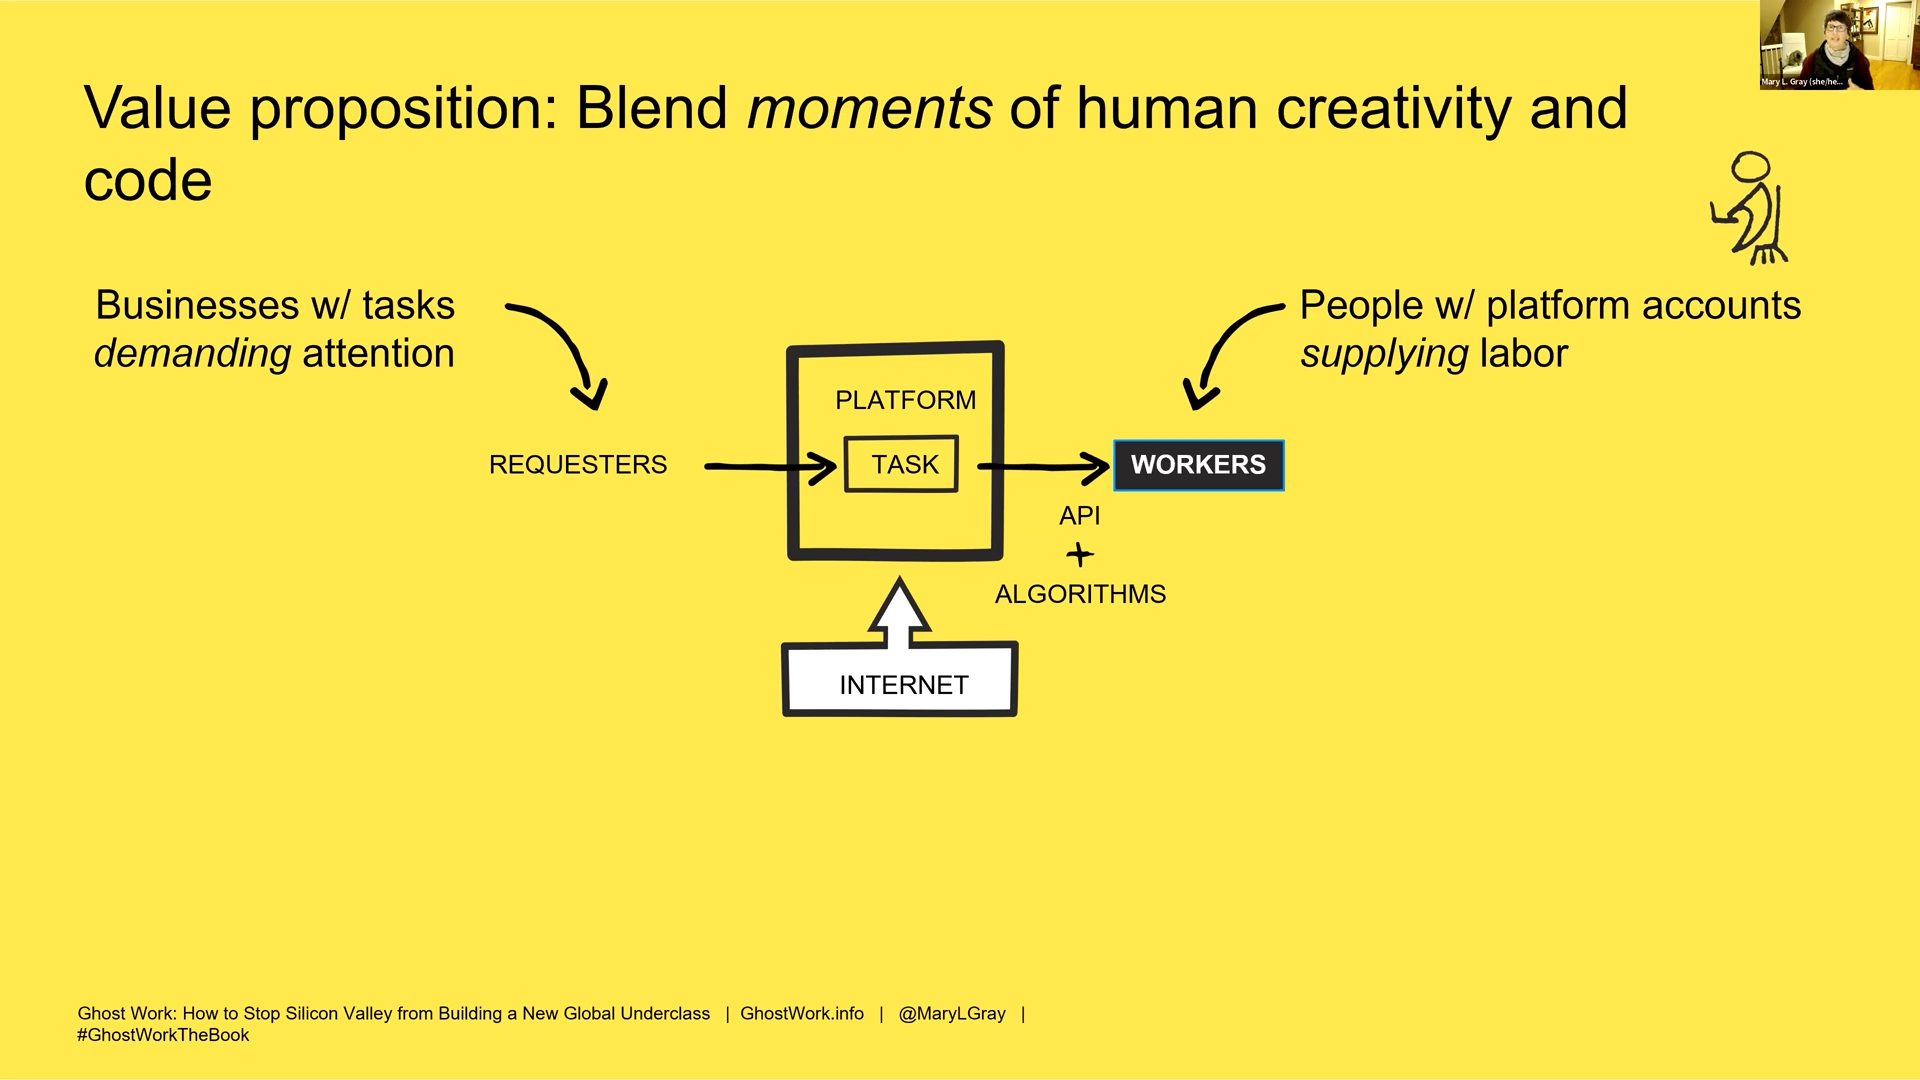
\includegraphics[width=\textwidth]{figures/videos/ghost_work/mixed.png}}

\only<+>{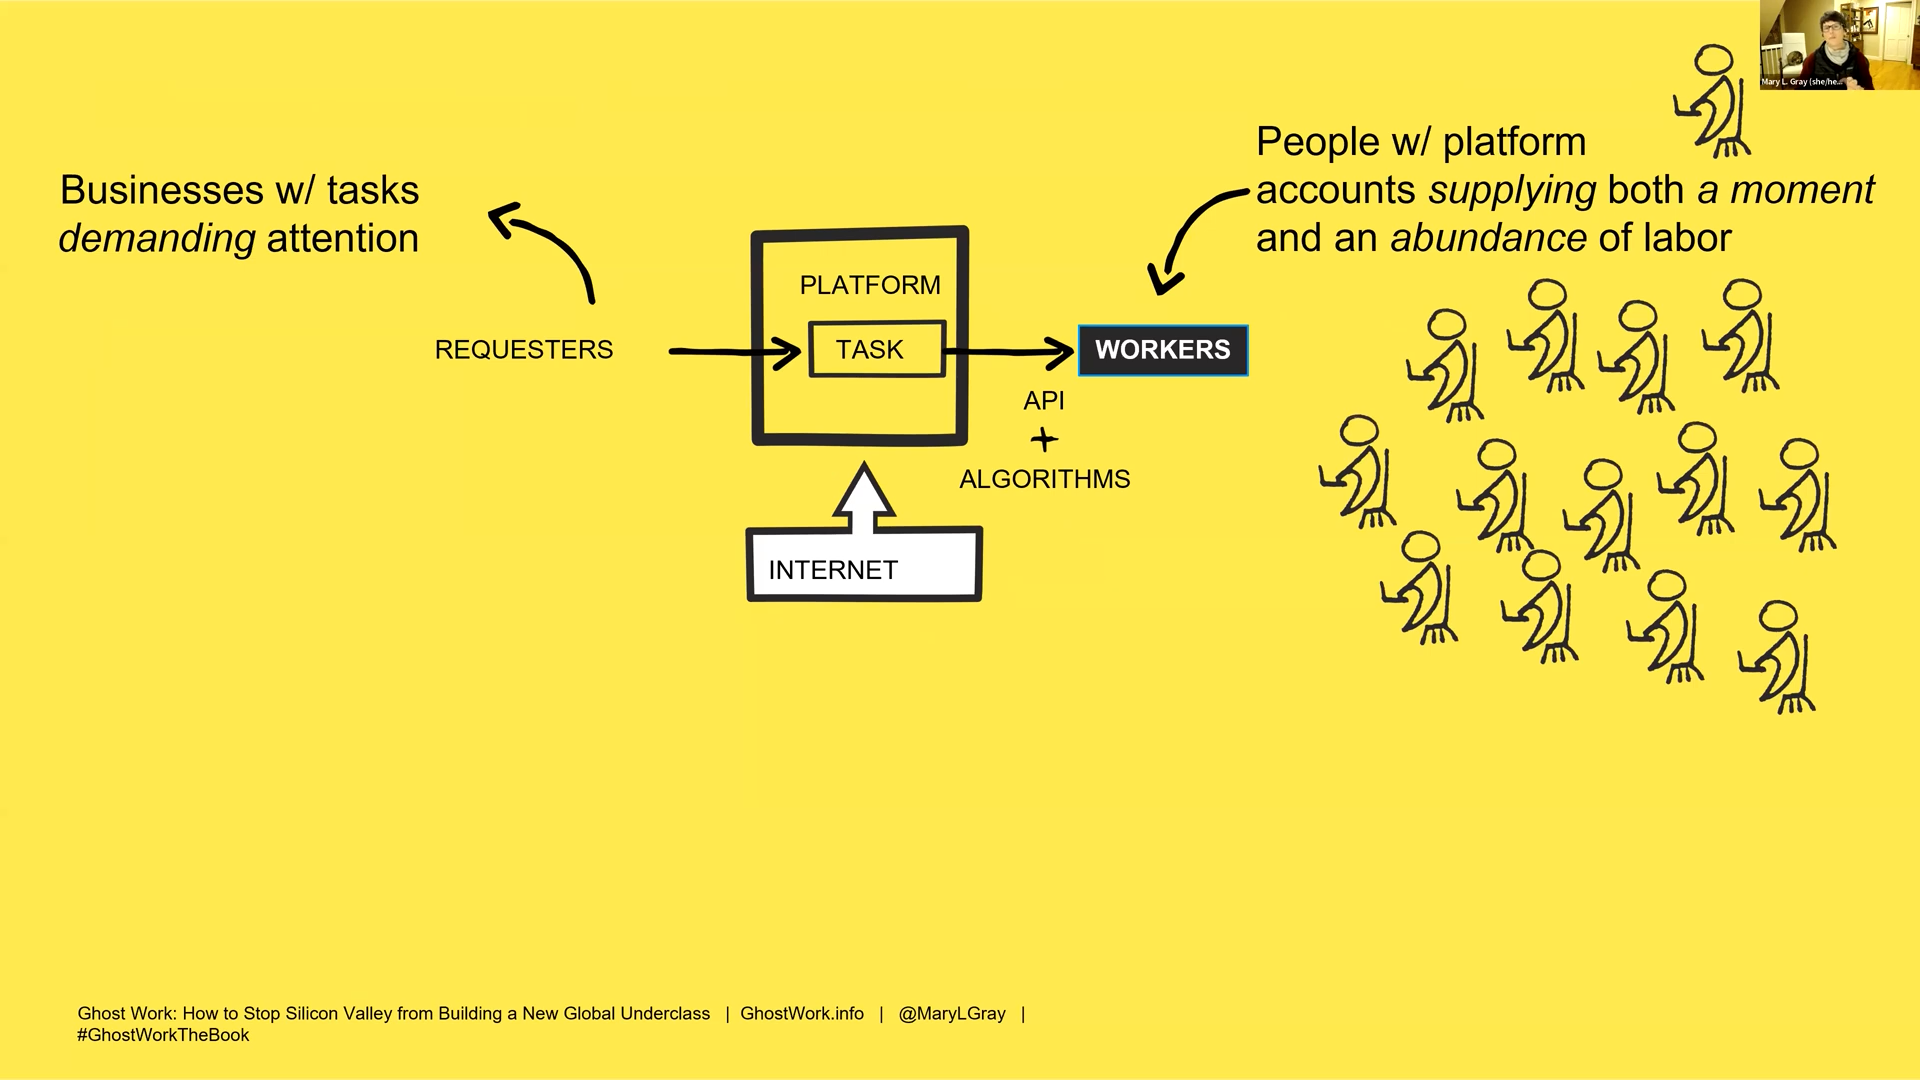
\includegraphics[width=\textwidth]{figures/videos/ghost_work/crowdwork.png}}

\only<+>{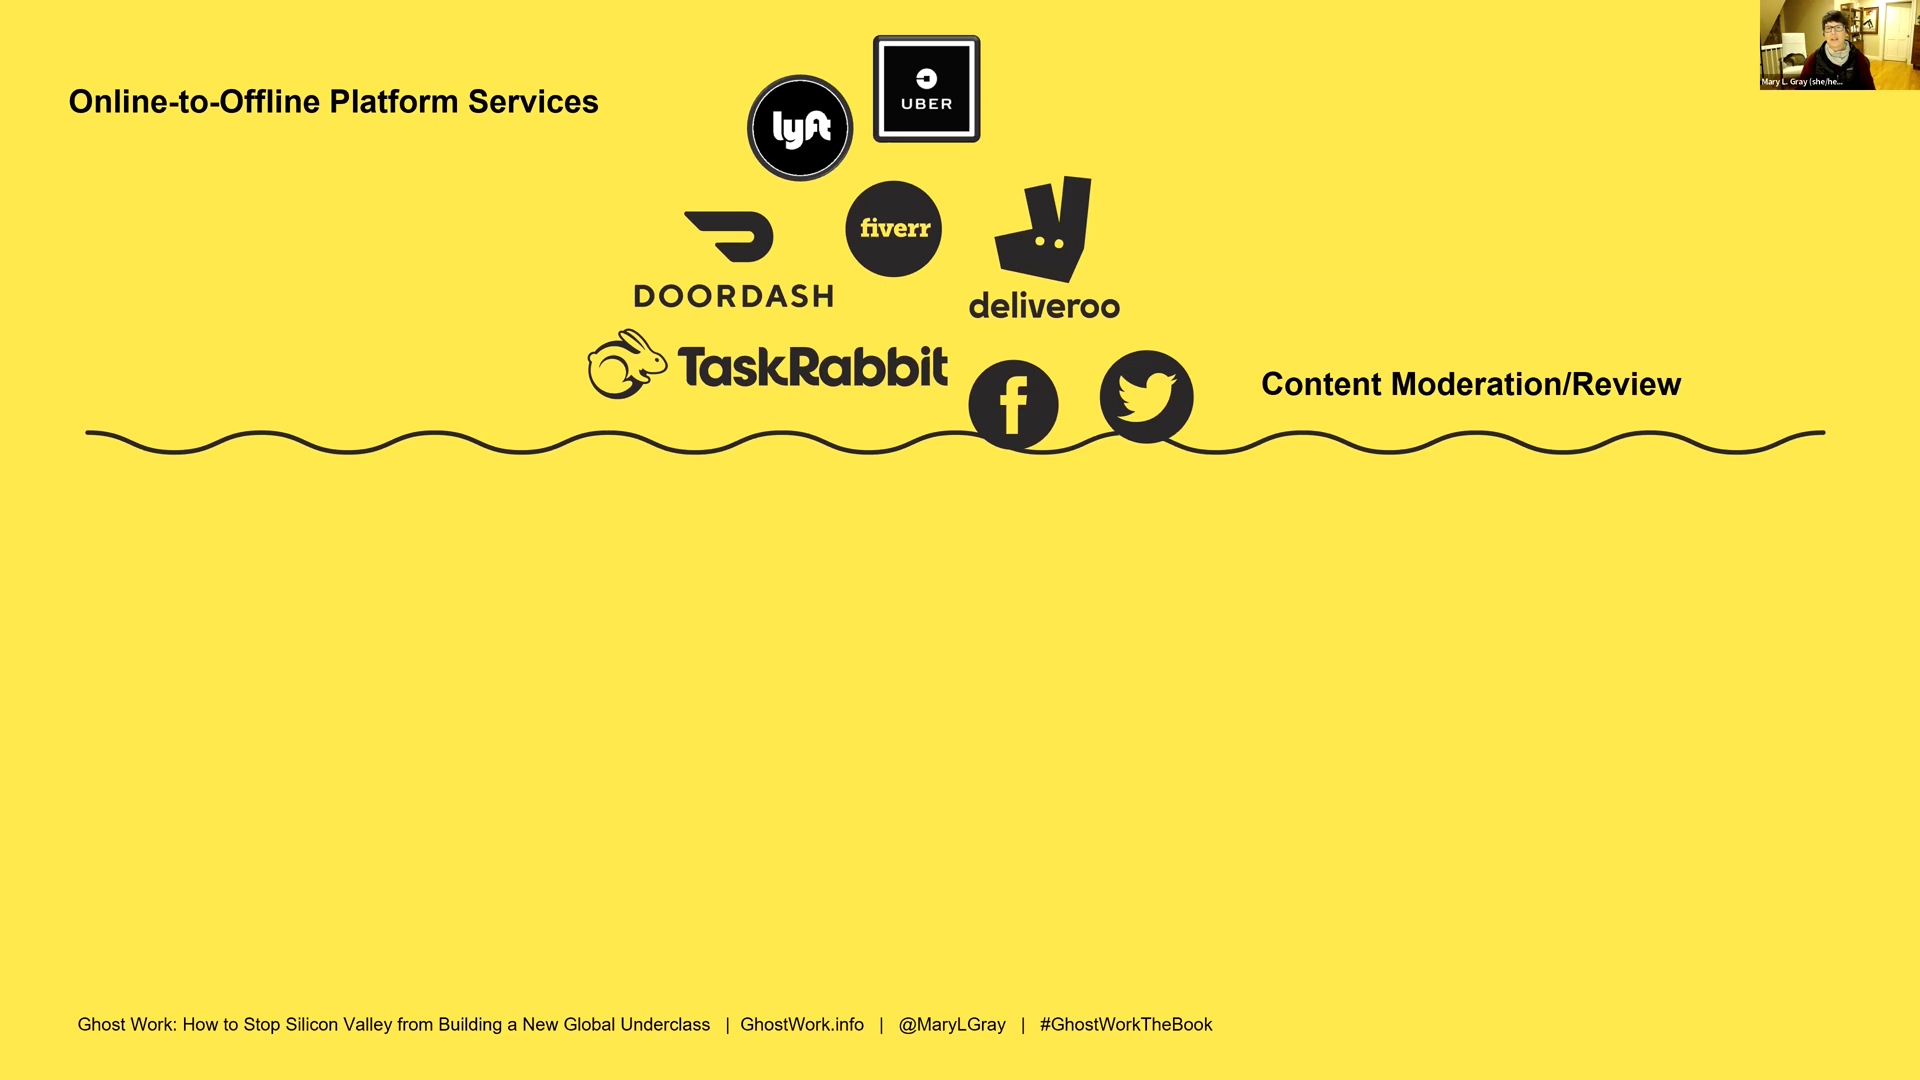
\includegraphics[width=\textwidth]{figures/videos/ghost_work/gig.png}}

\only<+>{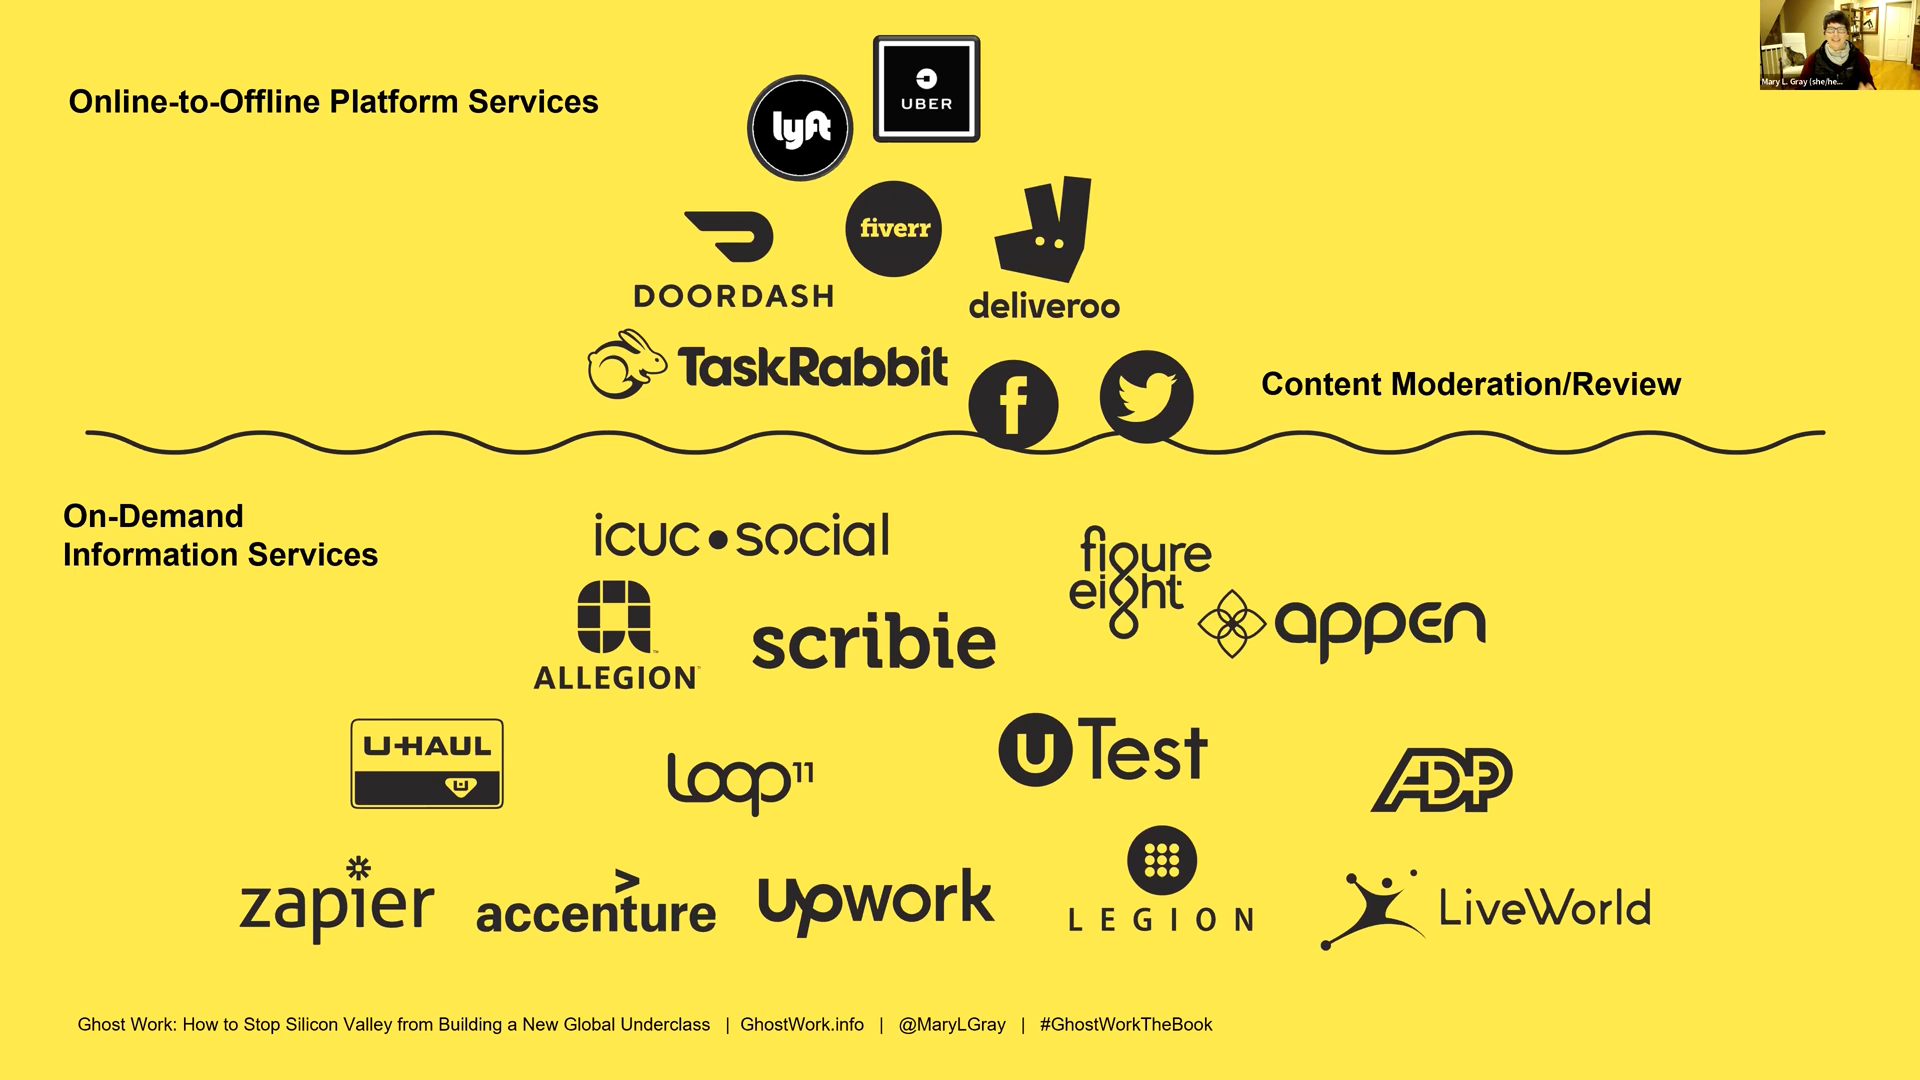
\includegraphics[width=\textwidth]{figures/videos/ghost_work/gigcrowd.png}}
\end{column}
\begin{column}{0.3\textwidth}
\includegraphics[width=\textwidth]{figures/books/ghost_work.jpeg}
\end{column}
\end{columns}

\end{frame}


\begin{frame}[plain]
    \only<+>{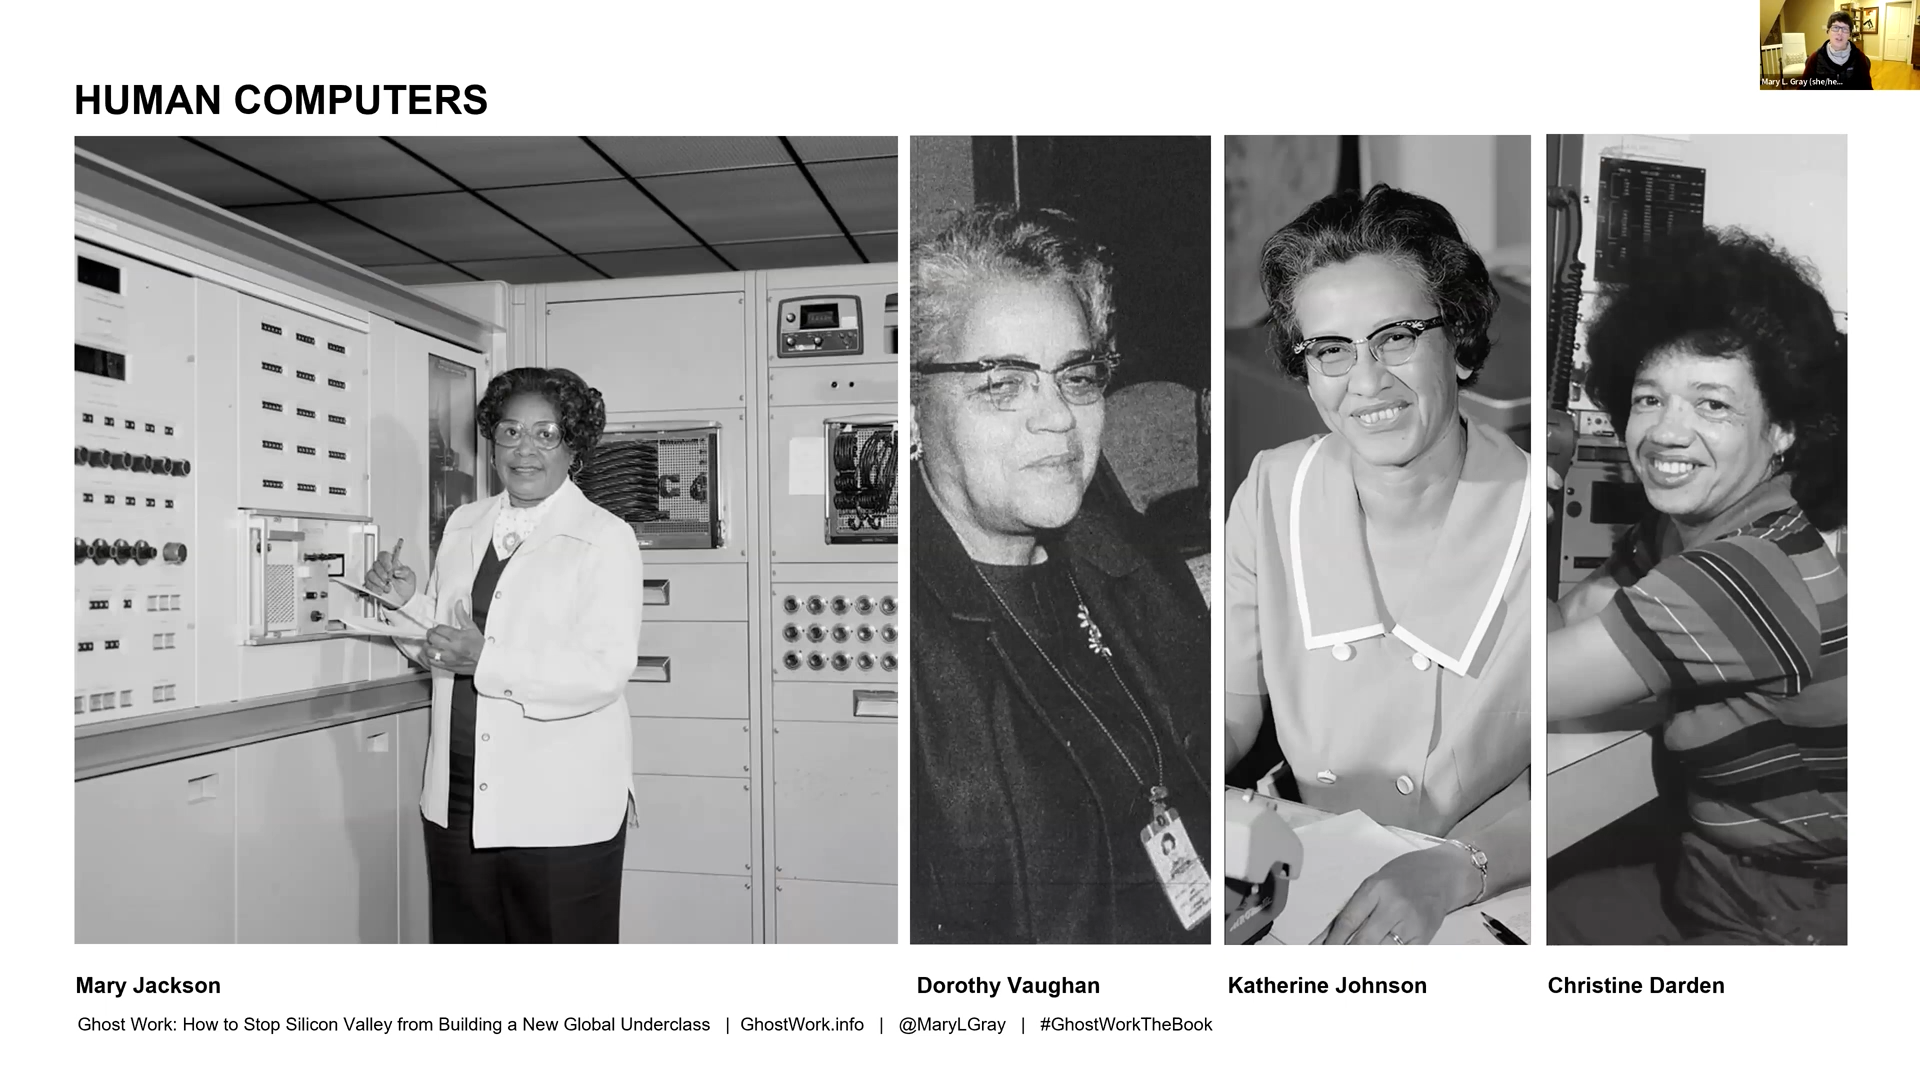
\includegraphics[width=\textwidth]{figures/videos/ghost_work/humanComp.png}}

    \only<+>{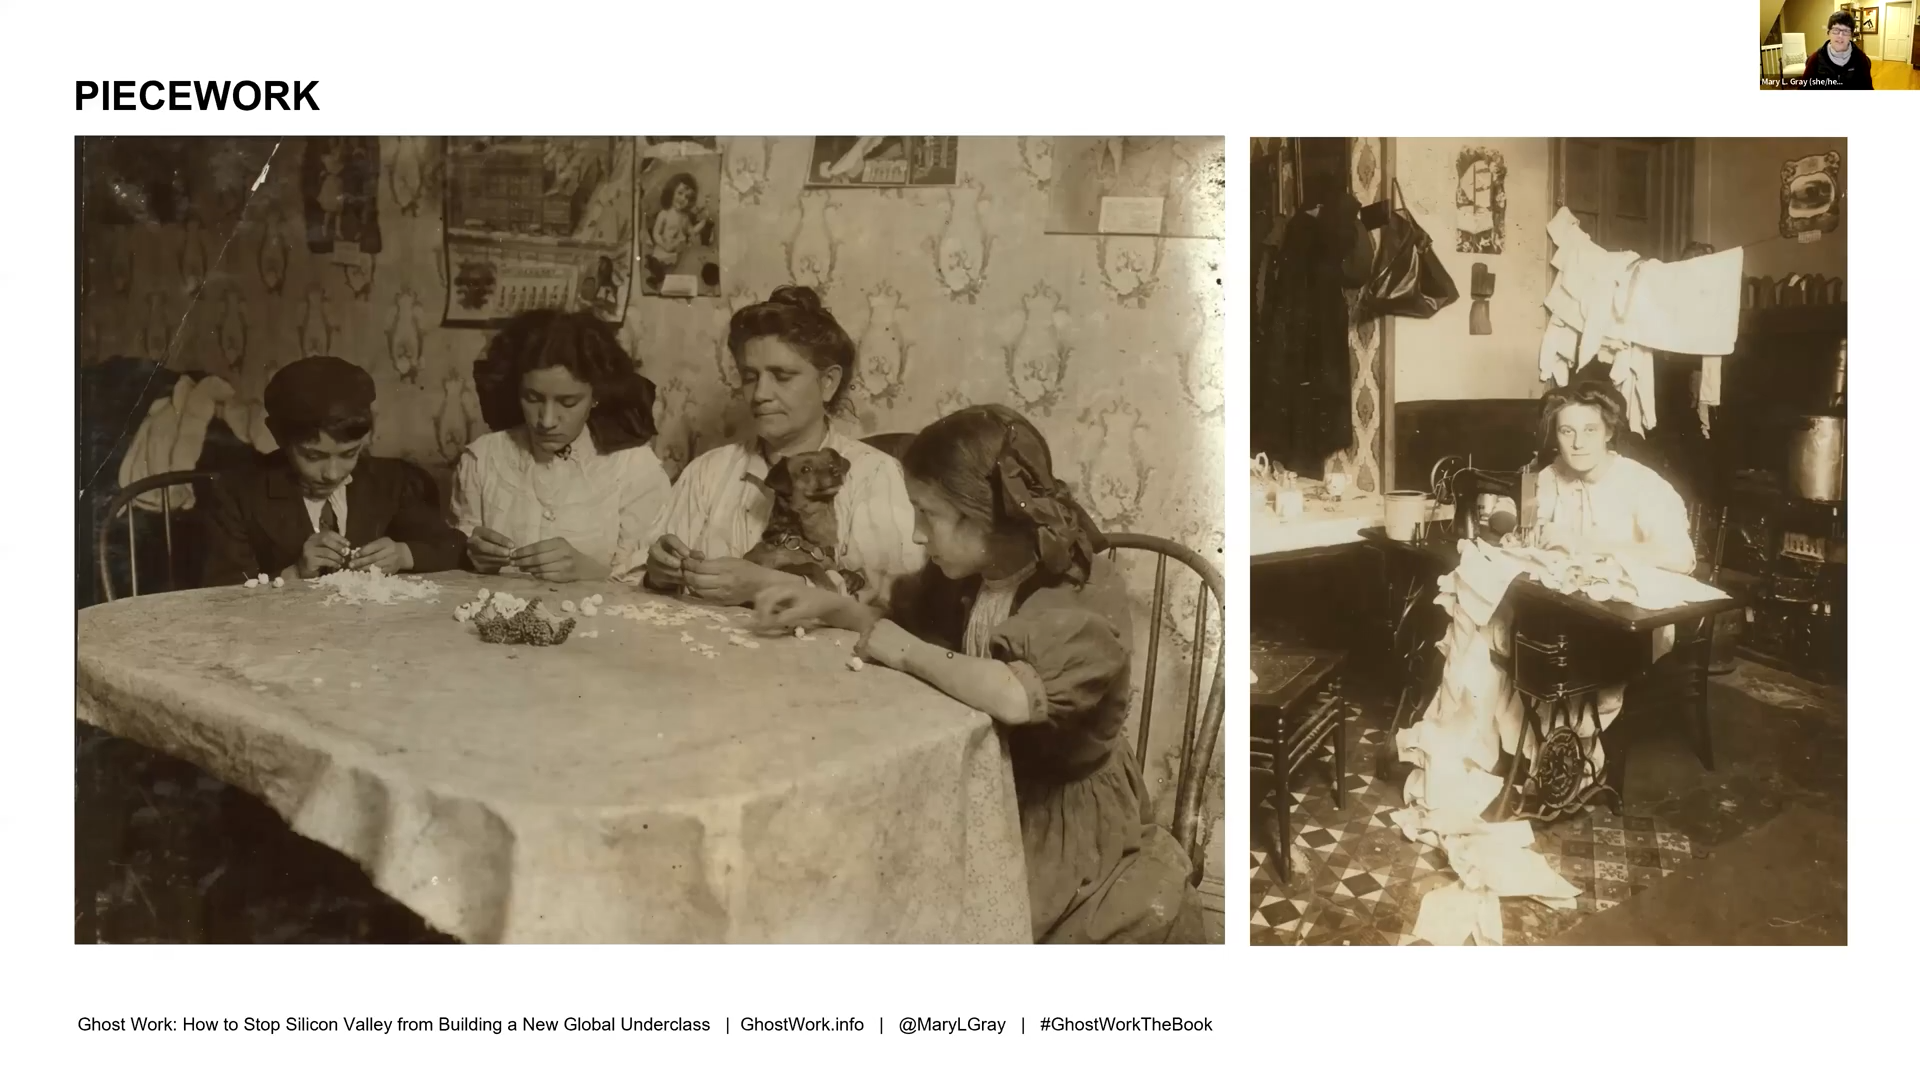
\includegraphics[width=\textwidth]{figures/videos/ghost_work/piecework.png}}

\end{frame}


\begin{frame}[plain]
\begin{columns}
\begin{column}{0.7\textwidth}
    \includegraphics[width=\textwidth]{figures/news/bullshit.png}
\end{column}
\begin{column}{0.3\textwidth}
    \includegraphics[width=\textwidth]{figures/books/bullshit_jobs.jpeg}
\end{column}
\end{columns}

\end{frame}


\begin{frame}[plain]
\centering
\visible<+->{How \emph{should} we talk about changes in labor?}

\end{frame}



\begin{frame}{questions}
    
\begin{itemize}
    \item How is the automation of this work being facilitated?
    \item Are those jobs replaced, shifted, or \dots what?
    \item How has work changed for the people doing work?
\end{itemize}

\end{frame}

\begin{frame}[plain,label=break]
\centering

\emph{break for group discussion, then reconvene}

\end{frame}



%%%%%%%%%%%%%%%%%%%%%%%%%%%%%%
%%%%%%%%%%%%%%%%%%%%%%%%%%%%%%
%%%%%%%%%%%%%%%%%%%%%%%%%%%%%%
%%%%%%%%%%%%%%%%%%%%%%%%%%%%%%
%%%%%%%%%%%%%%%%%%%%%%%%%%%%%%

\section{Social Good}

\begin{frame}[standout]

AI will allow us to scale social welfare

\end{frame}



\begin{frame}[plain]
\begin{columns}
\begin{column}{0.6\textwidth}
\only<+>{\includegraphics[width=\textwidth]{figures/videos/algos_at_work/at_work.png}}

\only<+>{\includegraphics[width=\textwidth]{figures/videos/algos_at_work/moneyballing.png}}

\end{column}
\begin{column}{0.4\textwidth}
\includegraphics[width=\textwidth]{figures/books/metrics.jpg}
\end{column}
\end{columns}
\end{frame}


\begin{frame}[plain]
\begin{columns}
\begin{column}{0.6\textwidth}
\centering
\only<+>{{\large \strong{Digital Poorhouse}}}

\only<+>{{\large {``You better watch what they're doing to us, because\\\vspace{1em} \strong{they're coming for you next}''}}}

\only<+>{\emph{primary goal: to increase self-determination}}

\only<+>{\emph{would this be tolerated if it weren't targeted at the poor?}}

\end{column}
\begin{column}{0.4\textwidth}
\includegraphics[width=\textwidth]{figures/books/automating_inequality.jpeg}
\end{column}
\end{columns}
\end{frame}

\begin{frame}[plain]

\begin{columns}
\begin{column}{0.5\textwidth}

\centering
\visible<2>{\emph{\small AI-enabled systems \dots are often introduced to the general public under the guise of offering service to disabled people \dots serving to normalize the presence of [invasive surveillance] in our day-to-day lives.}}

\end{column}
\begin{column}{0.5\textwidth}
    \includegraphics[width=\textwidth]{figures/papers/ainow.png}

\end{column}
\end{columns}


\end{frame}


\begin{frame}[standout]

Issues in social welfare?

\end{frame}


\begin{frame}[plain]

% \pnote{omit bias?}

\centering
\visible<+->{What are the issues that data-driven systems \emph{claim} to address?}

\visible<+->{What are the facets of welfare that data-driven systems \emph{actually} address?}

\end{frame}

\begin{frame}{questions}
\begin{itemize}
    \item What is \emph{supposedly} supported by the expansion of AI in a given context?
    \item How would this service differ if the human workforce were expanded?
    \item How does this algorithmic approach change the dynamic for people seeking resources?
\end{itemize}
\end{frame}



\againframe{break}



\begin{frame}[plain]


\end{frame}


\begin{frame}{bias, fairness, and justice}


\end{frame}


\end{document}
